%%% Optimal 125, 125_plot.dat, laufzeit: 3h
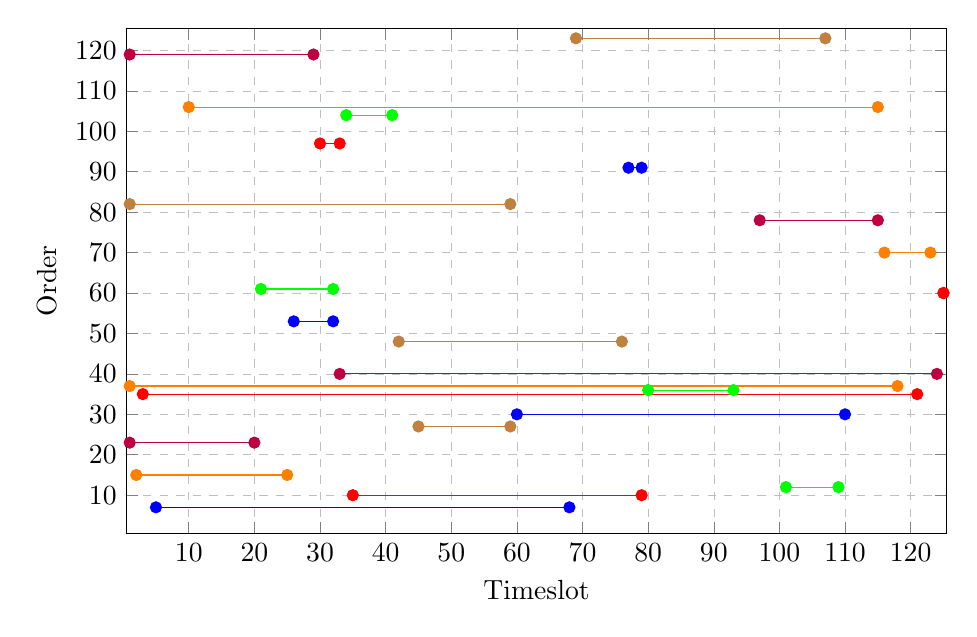
\begin{tikzpicture}
\begin{axis}[
   % title={Optimal Schedule},
    xlabel={Timeslot},
    ylabel={Order},
    xmin=0.5, xmax=125.5, 
    ymin=0.5, ymax=125.5, 
    xtick={10,20,30,40,50,60,70,80,90,100, 110, 120},
    ytick={10,20,30,40,50,60,70,80,90,100, 110, 120},
    grid=both,
    grid style={line width=.1pt, draw=gray!10},
    major grid style={line width=.2pt, draw=gray!50},
    legend pos=north east,
    ymajorgrids=true,
    xmajorgrids=true,
    grid style=dashed,
    width=12cm,
    height=8cm,
]
\addplot[color=blue, mark=*] coordinates {(5, 7) (68, 7)};
\addplot[color=red, mark=*] coordinates {(35, 10) (79, 10)};
\addplot[color=green, mark=*] coordinates {(101, 12) (109, 12)};
\addplot[color=orange, mark=*] coordinates {(2, 15) (25, 15)};
\addplot[color=purple, mark=*] coordinates {(1, 23) (20, 23)};
\addplot[color=brown, mark=*] coordinates {(45, 27) (59, 27)};
\addplot[color=blue, mark=*] coordinates {(60, 30) (110, 30)};
\addplot[color=red, mark=*] coordinates {(3, 35) (121, 35)};
\addplot[color=green, mark=*] coordinates {(80, 36) (93, 36)};
\addplot[color=orange, mark=*] coordinates {(1, 37) (118, 37)};
\addplot[color=purple, mark=*] coordinates {(33, 40) (124, 40)};
\addplot[color=brown, mark=*] coordinates {(42, 48) (76, 48)};
\addplot[color=blue, mark=*] coordinates {(26, 53) (32, 53)};
\addplot[color=red, mark=*] coordinates {(125, 60) (125, 60)};
\addplot[color=green, mark=*] coordinates {(21, 61) (32, 61)};
\addplot[color=orange, mark=*] coordinates {(116, 70) (123, 70)};
\addplot[color=purple, mark=*] coordinates {(97, 78) (115, 78)};
\addplot[color=brown, mark=*] coordinates {(1, 82) (59, 82)};
\addplot[color=blue, mark=*] coordinates {(77, 91) (79, 91)};
\addplot[color=red, mark=*] coordinates {(30, 97) (33, 97)};
\addplot[color=green, mark=*] coordinates {(34, 104) (41, 104)};
\addplot[color=orange, mark=*] coordinates {(10, 106) (115, 106)};
\addplot[color=purple, mark=*] coordinates {(1, 119) (29, 119)};
\addplot[color=brown, mark=*] coordinates {(69, 123) (107, 123)};

\end{axis}
\end{tikzpicture}